\documentclass[11pt, a4paper, german]{article}
\pagestyle{plain}

\usepackage[german]{babel}
\usepackage{amsmath}
\usepackage{amsthm}
\usepackage{amssymb}
\usepackage{graphicx}
\usepackage{tikz}
\usepackage[utf8]{inputenc}
\usepackage{caption}
\usepackage{subcaption}
\usepackage[colorlinks=true, pdfborder={0 0 0}, linkcolor=blue, citecolor=blue]{hyperref}

\newcommand{\HRule}{\rule{\linewidth}{0.5mm}}
\setlength{\parindent}{0cm}

\begin{document}
\begin{titlepage}

\begin{center}


% Oberer Teil der Titelseite:

\textsc{\LARGE Projektgruppe Angewandte Softwaretechnologie}\\[1.5cm]

\textsc{\Large Sommersemester 2015}\\[0.5cm]

\HRule \\[0.4cm] { \huge \bfseries DLVC Taverne}\\[0.2cm]
{\large \bfseries Ein Handbuch}\\[0.4cm]

\HRule \\[1.5cm]

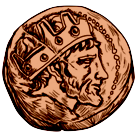
\includegraphics[width=0.6\textwidth]{./Logo3_1.png}\\[1cm]

\begin{minipage}{0.4\textwidth} \begin{flushleft} \large \emph{Author:}\\ Projektgruppe DLVC Taverne \end{flushleft} \end{minipage} \hfill \begin{minipage}{0.4\textwidth} \begin{flushright} \large \emph{Supervisor:} \\ Günther Kniesel \end{flushright} \end{minipage}

\vfill

{\large \today}

\end{center}

\end{titlepage}
\clearpage

\tableofcontents
\pagebreak
\section{Allgemeine Informationen}
Die Zielsetzung von \textit{DLVC Taverne} ist es, Spielleitern im Pen\&Paper-Rollenspiel 'Die Legenden von Cystaron' (DLVC) ihre Aufgabe zu erleichtern. Insbesondere im Kampf sollen langwierige Würfeleien und Rechnungen vonseiten des Spielleiters vermieden werden.
\subsection{Hinweis}
Dieses Handbuch geht davon aus, dass dem Leser die Regeln von DLVC bekannt sind. 
\subsection{Technische Voraussetzungen}
\textit{DLVC Taverne} ist auf Windows ausgelegt. Auf anderen Betriebssystemen kann es zu Darstellungsmängeln kommen. \\
Zudem wird Java in Version von mindestens 1.8.0\_40 benötigt.
\subsection{Arbeitsgruppe}
Das Programm \textit{DLVC Taverne} ist 2015 im Rahmen der Projektgruppe 'Angewandte Softwaretechnologie' unter der Leitung von Dr. Kniesel entstanden. Die Entwickler waren:
\begin{itemize}
	\item[] Britta Heymann
	\item[] Andreas Kofer
	\item[] Nooshin Naghavi
	\item[] Boris Prochnau
\end{itemize}

\newpage
\section{Das Hauptmenü}
Das Hauptmenü besteht aus zwei vertikal getrennten Bereichen, den Buttons für die Hauptfunktionen und der Gruppenauswahl (siehe Abb. \ref{fig:Hauptmenue1}). Außerdem findet sich (wie auf fast jedem Fenster) ein Hilfe Button am rechten unteren Rand, welcher über das aktuelle Fenster informieren kann.
\begin{figure}
\centering
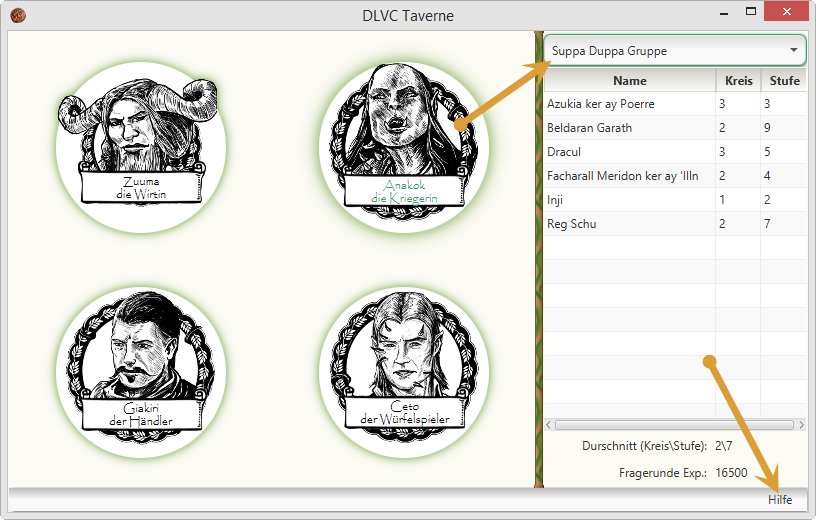
\includegraphics[width=1\linewidth]{Bilder/Hauptmenue1}
\caption{Hauptmenü mit Gruppenauswahl und Hlife Button}
\label{fig:Hauptmenue1}
\end{figure}

\subsection{Button Bereich}
%\textbf{Button Bereich:}\\
Im linken Bereich finden sich vier Buttons, um auf die Grundfunktionen des Programm zuzugreifen.
\begin{itemize}
	\item[] \textbf{Zuuma, die Wirtin (Charaktermanager)}: Hier können Spieler- und Nichtspielercharaktere angelegt, sowie Abenteuergruppen verwaltet werden.
	\item[] \textbf{Anakok, die Kriegerin (Kampf)}: Führt zu einer Teilnehmerauswahl für die Teilnehmer des Kampfes (Spieler und Gegner). Anschließend kann ein Kampfhelfer für den Kampf gestartet werden.
	\item[] \textbf{Giriki, der Händler}: Hier können alle Gegenstände und Ausrüstungsteile erstellt, gesucht und anderweitig verwaltet werden.
	\item[] \textbf{Ceto, der Würfelspieler (Würfeln)}: Hier können diverse Würfelwürfe simuliert werden.
\end{itemize}

\subsection{Gruppenauswahl}\label{subsection:gruppenauswahl}
Im rechten Bereich findet sich die Gruppenauswahl. Jede zuvor im Charaktermanger zusammengestellte Gruppe kann in der Liste ganz oben ausgewählt werden, woraufhin alle Mitglieder mit Kreis und Level angezeigt werden.\\
Die Auswahl einer Gruppe im Hauptmenü führt dazu, dass diese die Standardgruppe in der Abenteuerverwaltung und bei Kämpfen ist.

\newpage

\section{Charaktermanager (Zuuma, die Wirtin)}
Um den Kampfhelfer zu nutzen, müssen \textit{DLVC Taverne} Spieler- und Nichtspielercharaktere bekannt sein. Dafür ist der Charaktermanager zuständig. Er teilt sich in die drei Tabs \textbf{Gruppen}, \textbf{Spielercharaktere} und \textbf{Nichtspielercharaktere}.

\subsection{Der Gruppenmanager}
Der Gruppenmanager ermöglicht das Speichern von Abenteuergruppen. Diese können dann schnell bei Neustart wiederverwendet und angepasst werden.\\
Große Vorteile sind, dass man im Kampf standardmäßig die entsprechenden Mitglieder der Gruppe als Teilnehmer hat und durch einmalige Auswahl im Hauptmenü stets verfolgen kann, welche Stufe die Spieler haben und so bemerkt, wenn sie geändert werden müssen (siehe Abschnitt \ref{subsection:gruppenauswahl}).\\
\begin{figure}
\centering
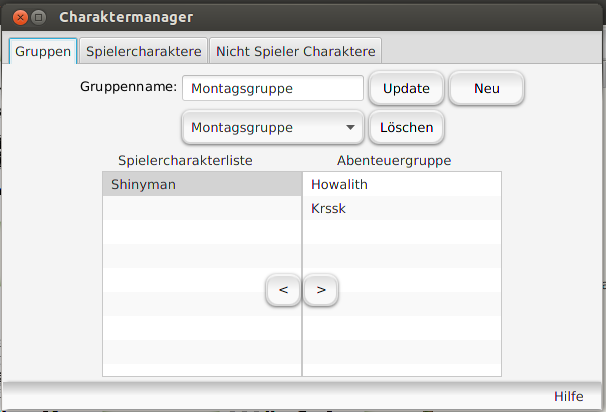
\includegraphics[width=1\linewidth]{Bilder/Gruppenmanager}
\caption{Der Gruppenmanager. Die Spielercharaktere auf der rechten Seite gehören zu der ausgewählten Gruppe.}
\label{fig:Gruppenmanager}
\end{figure}

Der Gruppenmanager besteht im Wesentlichen aus zwei Listen und dem oberen Bereich zum Anpassen der Gruppennamen.\\

\textbf{Anlegen neuer Gruppen}: Dazu muss ein Name in das obere Textfeld geschrieben und mit dem Button '\textbf{Neu}' oder mit der 'Enter'-Taste bestätigt werden.\\

\textbf{Ändern einer Gruppe}: Existieren bereits Gruppen, so kann man sie in der unter dem Textfeld liegenden Box auswählen. Der Name erscheint dann im Textfeld und kann editiert und mit einem Klick auf den Button '\textbf{Update}' gespeichert werden. \\

\textbf{Löschen einer Gruppe}: Mit dem '\textbf{Löschen}'-Button wird die selektierte Gruppe gelöscht. \textit{Hinweis}: Dies löscht nur die Zuordnungen der Spielercharaktere zu der Gruppe, nicht die Spielercharaktere selbst.\\

Um Spielercharaktere zu einer Gruppe hinzuzufügen oder zu entfernen, muss die entsprechende Gruppe selektiert werden. Durch Klicken auf die Pfeilbuttons wird die neue Aufteilung herbeigeführt und direkt abgespeichert.

\subsection{Der Spielercharaktermanager}\label{subsection:Spielercharaktermanager}
Im Spielercharaktermanager werden die kampfrelevanten Eigenschaften von Spielercharakteren abgespeichert. 
Er ist dafür in die drei Untertabs 'Details', 'Waffen\&Fähigkeiten' und 'Ausrüstung' aufgeteilt.\\
\begin{figure}[h!]
\centering
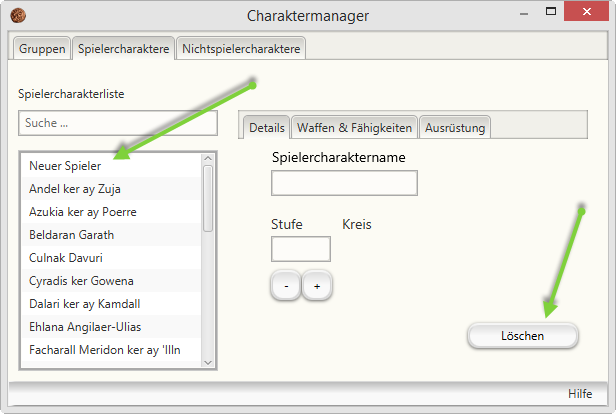
\includegraphics[width=1\linewidth]{Bilder/Charaktermanager1}
\caption{Neuen Spieler auswählen und Löschen Button}
\label{fig:Charaktermanager1}
\end{figure}

\textbf{Erstellen neuer Spielercharaktere}: Dazu muss der Eintrag 'Neuer Spieler' in der Spielercharakterliste ausgewählt werden (siehe Abb. \ref{fig:Charaktermanager1}). Durch Abändern der Standardwerte und das Drücken der 'Enter'-Taste wird der neue Spieler gespeichert und erscheint in der Liste am linken Rand.\\

\textbf{Ändern von Spielercharakteren}: Das Editieren eines bereits bestehenden Charakters funktioniert auf dieselbe Art und Weise, nur, dass man zunächst den zu ändernden Charakter aus der Liste wählt.\\

\textbf{Löschen von Spielercharakteren}: Um einen ausgewählten Spielercharakter zu löschen, drückt man lediglich den 'Löschen'-Button im Tab 'Details (siehe Abb. \ref{fig:Charaktermanager1})'.


\subsubsection{Die 3 Untertabs für Spielercharakter-Eigenschaften}
\textbf{Details:} Dieser Tab ist sehr simpel. Er enthält lediglich den Namen des Spielers, seinen Kreis und seine Stufe. Kreis und Stufe werden durch einschrittige Veränderungen mithilfe der '+'- und '-'-Buttons editiert. Zudem kann man in diesem Tab den Spielercharakter ganz \textbf{löschen}.\\

\textbf{Waffen\&Fähigkeiten}: Hier können dem Spielercharakter Waffen hinzugefügt werden, die er im Kampf auswählen kann. \\
Die Grundstruktur ist dieselbe wie die des Spielercharaktermanagers selbst: Am linken Rand ist eine Waffenliste mit einem Eintrag '\textbf{Neue Waffe}', rechts können Eigenschaften manipuliert und die selektierte Waffe gelöscht werden.
\begin{figure}[h]
\centering
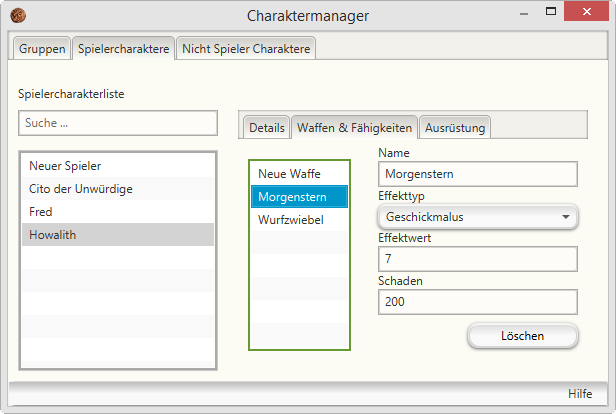
\includegraphics[width=1\linewidth]{Bilder/Charaktermanager_Spieler1}
\caption{Der Waffen\&Fähigkeiten-Tab}
\label{fig:Charaktermanager_Spieler1}
\end{figure}

Jede Waffe kann neben einen Namen und einem Schadenwert auch einen Effekt besitzen. Dafür wird zunächst der Effekttyp ausgewählt und dann der Effektwert definiert. Die Bedeutung des Effektwerts hängt vom Effekttyp ab (siehe Abschnitt \ref{Abschnitt: Effekte}): \begin{itemize}
\item[] \textit{Rüstungsunabhängig} benötigt keinen Effektwert.
\item[] \textit{Stärkemalus} spezifiziert einen absoluten Wert, der von der Stärke des Gegners subtrahiert wird.
\item[] \textit{Geschickmalus} spezifiziert einen absoluten Wert, der vom Geschick des Gegners subtrahiert wird.
\item[] \textit{Schaden an allen Gegnern} benötigt keinen Effektwert.
\end{itemize}

\textbf{Ausrüstung}: Hier wird die Rüstung des Spielercharakters spezifiziert. Dies beinhaltet natürlich den Rüstungs-, Helm- und Schildwert (DefR, DefH, DefS). Zusätzlich kann die Rüstung Effekte verursachen, siehe Abbildung \ref{fig:Spielercharaktermanager3}. Wie bei Waffen können Geschick- und Stärkemalus eingetragen werden. Hat die Rüstung keinen solchen Malus, entspricht diese einem Wert von 0. Zusätzlich kann die Rüstung eines Spielers ihm mehr Erfahrung im Kampf einbringen. Diese Steigerung wird in Prozent angegeben und später im Kampfende gesondert angezeigt, siehe Abschnitt \ref{Abschnitt:Kampfende}.\\
\begin{figure}
\centering
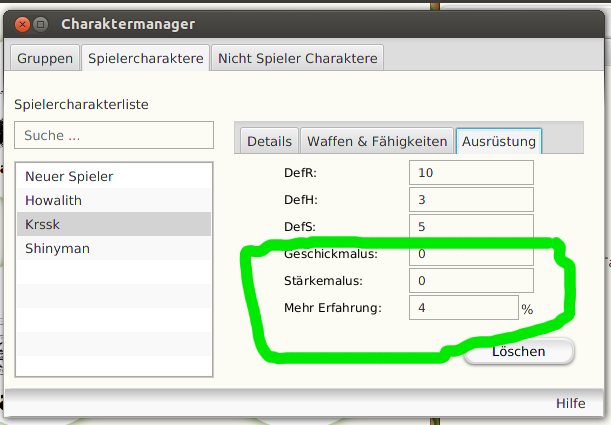
\includegraphics[width=1\linewidth]{Bilder/Spielercharaktermanager3}
\caption{Der Ausrüstungstab. Die Werte für Effekt sind markiert. Eine 0 heißt hier, dass die Rüstung diesen Effekt nicht besitzt.}
\label{fig:Spielercharaktermanager3}
\end{figure}

In jedem Tab führt ein Druck auf die 'Enter'-Taste zur Speicherung der Charakterwerte.


\subsubsection{Effekte von Rüstung und Waffen} \label{Abschnitt: Effekte}
Eine \textbf{Waffe} kann höchstens einen der folgenden Effekte besitzen:
\begin{itemize}
\item[] \textit{Rüstungsunabhängig}: Benötigt einen Würfelwurf. Der so geworfene Schaden wird rüstungsunabhängig am Gegner verursacht. Dieser Effekt dient nur zur Erinnerung; da der konkrete Schaden abhängig vom Würfel ist, muss er manuell eingegeben werden, siehe Abschnitt \ref{Abschnitt:standardkampf}: Lebenspunkte reduzieren.
\item[] \textit{Stärkemalus} spezifiziert einen absoluten Wert, der von der Stärke des Gegners subtrahiert wird, wenn dieser eine Stärkeprobe im Kampf macht. Dies wird vom Programm geleistet, wenn der entsprechende Spieler in der Spielerrunde ausgewählt ist, siehe Abschnitt \ref{Abschnitt:staerkewurf}.
\item[] \textit{Geschickmalus} spezifiziert einen absoluten Wert, der vom Geschick des Gegners subtrahiert wird, wenn dieser blockt oder angreift. Dies wird vom Programm geleistet. Beim Blocken muss der entsprechende Spieler ausgewählt sein, siehe Abschnitt \ref{Abschnitt:standardkampf}: Blocken.
\item[] \textit{Schadet an allen Gegnern} besagt, dass der Spieler die Fähigkeit hat, Schaden auf allen Gegner gleichzeitig auszulösen. Dann erscheint in der Spielerrunde (Abschnitt \ref{Abschnitt:aoe}) ein entsprechender Button.
\item[] \textit{Schadet an allen Gegnern rüstungsunabhängig} Genauso wie 'Schadet allen Gegnern', nur, dass die Rüstung der Gegner ignoriert wird. Somit hängt die Wirkung des eben erwähnten Buttons auch vom genauen Effekt ab.
\end{itemize}
Jede \textbf{Rüstung} kann zusätzlich folgende Effekte haben:
\begin{itemize}
\item[] \textit{Stärkemalus}: Wie für Waffen.
\item[] \textit{Geschickmalus}: Wie für Waffen.
\item[] \textit{Mehr Erfahrung}: Prozentsatz, wie viele Erfahrungspunkte mehr der entsprechende Spieler bekommt. Wird automatisch beim Kampfende angewandt, siehe Abschnitt \ref{Abschnitt:Kampfende}: Die Erfahrungpunkte.
\end{itemize}
\textbf{Soll einer der Rüstungseffekt nicht vorhanden sein}, setzt man seinen Wert auf 0.

\subsection{Der Nichtspielercharakter-Manager}
Im Nichtspielercharakter-Manager werden potentielle Gegner der Abenteuergruppen verwaltet. \\

Von der Bedienung her funktioniert der Nichtspielercharakter-Manager fast identisch zum Spielermanager, siehe Abschnitt \ref{subsection:Spielercharaktermanager}. Er besitzt lediglich andere Tabs und eine zusätzliche Filterfunktion.\\

Mithilfe der Filterfunktion ist es leicht möglich, \textbf{Nichtspielercharaktere eines bestimmten Kreises zu finden}: Es werden stets die Typen angezeigt, deren Kreise ausgewählt sind, siehe Abbildung \ref{fig:Nichtspielertypmanager1}.
\begin{figure}
\centering
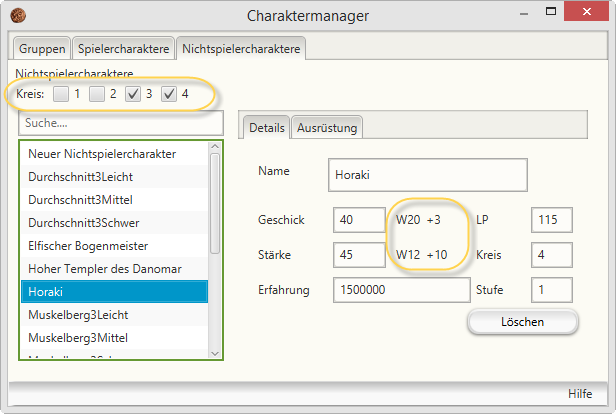
\includegraphics[width=1\linewidth]{Bilder/Nichtspielertypmanager1}
\caption{Der Nichtspielercharakter-Manager. Markiert sind die Filterfunktion und die Anzeige der zu den Geschick und Stärke passenden Würfelwerte.}
\label{fig:Nichtspielertypmanager1}
\end{figure}


\subsubsection{Die 2 Untertabs für Nichtspielercharakter-Eigenschaften}
Da für Nichtspielercharaktere im Kampf andere Werte wichtig sind als für Spielercharaktere, hat der Nichtspielercharakter-Manager nur die beiden Tabs 'Details' und 'Ausrüstung'.\\

Der Tab \textbf{Details} enthält wie bei den Spielercharakteren Name, Stufe und Kreis des Charakters. Auch hier kann ein Charakter \textbf{gelöscht} werden. 
Zusätzlich können die Werte Geschick, Stärke, Erfahrung und LP gesetzt werden.\\
 Geschick und Stärke bestimmen, wie sich der Gegner im Kampf verhält. Wenn eine dieser Zahlen durch 'Enter' bestätigt wird, updaten sich auch die daneben angezeigten Würfel. 
Sie zeigen an, welche Würfelwürfe intern simuliert werden. LP bestimmt die Lebenspunkte eines Charakters, Erfahrung gibt an, wie viele Erfahrungspunkte eine Instanz dieses Charakters einbringt.\\
\begin{figure}
\centering
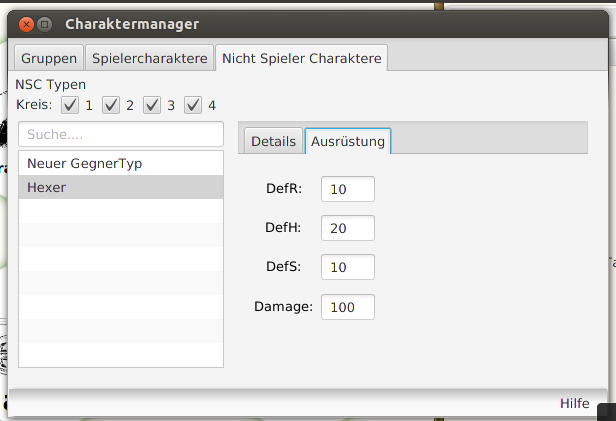
\includegraphics[width=1\linewidth]{Bilder/Nichtspielertypmanager2}
\caption{Der Ausrüstung-Tab}
\label{fig:Nichtspielertypmanager2}
\end{figure}

Im \textbf{Ausrüstung}-Tab werden erneut DefR, DefH und DefS angegeben, siehe Abschnitt \ref{subsection:Spielercharaktermanager}. 
Da einem Nichtspielercharakter eine feste Waffe zugewiesen ist, wird hier zudem der Schaden dieser Waffe festgelegt.

\clearpage
\section{Der Kampf (Anakok, die Kriegerin)}\label{Abschnitt:Kampf}
Der Kampf fängt mit einer Teilnehmerauswahl an. Erst, wenn man dort auf 'Kampf' klickt, öffnet sich das eigentliche Fenster, dass aus den drei Tabs \textbf{Gegnerrunde}, \textbf{Spielerrunde} und \textbf{Kampfende} besteht.
\subsection{Die Teilnehmerauswahl}
Die Teilnehmerauwahl gliedert sich in 4 Tabellen. Die oberen beiden Tabellen beziehen sich auf Spielercharaktere und die unteren beiden auf Gegner. Die Tabellen auf der rechten Seite zeigen an, wer gerade ausgewählt ist, um am Kampf teilzunehmen.\\

\textbf{Spieler zum Kampf hinzufügen.} Am einfachsten lässt sich eine gesamte Abenteuergruppe zum Kampf hinzufügen. Dies funktioniert mit der links oben verankerten Dropdownliste. Einzelne Spieler können dann mithilfe der Pfeilbuttons wieder aus dem Kampf entfernt werden. Alternativ wählt man keine Gruppe aus und fügt die Spieler einzeln von der linken Tabelle in die recht ein. Zur Vereinfachung existiert hier eine Suchbox.\\
\begin{figure}
\centering
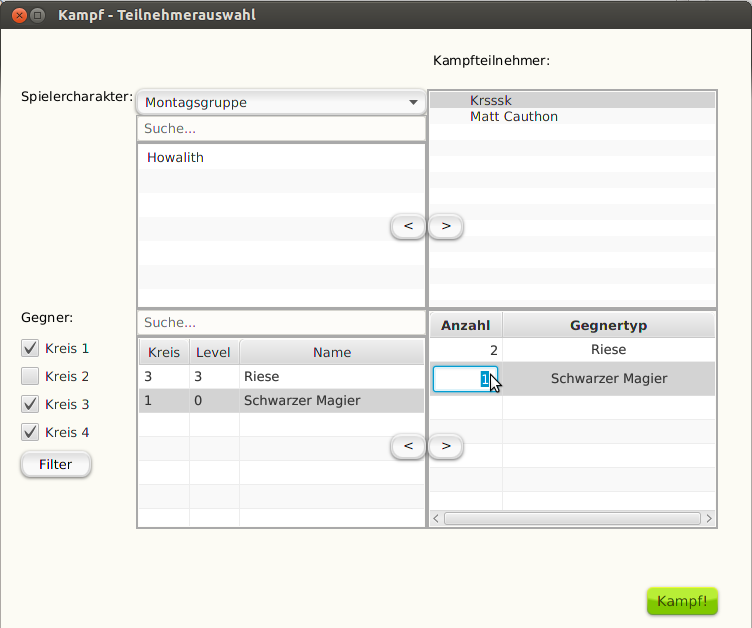
\includegraphics[width=.7\linewidth]{Bilder/Teilnehmerauswahl}
\caption{Die Teilnehmerauswahl. Rechts stehen die aktuell ausgewählten Kampfteilnehmer.\\ Man sieht, wie man die Anzahl der Gegner manuell editieren kann.}
\label{Abbildung: Teilnehmerauswahl}
\end{figure}

\textbf{Gegner zum Kampf hinzufügen.} Mithilfe des Filterbuttons am linken Rand können die Gegner nach Kreis angezeigt werden. Als zusätzliche Hilfestellung existiert eine Suchbox. Weiterhin kann man die Tabelle durch klicken auf die Spaltennamen nach Kreis, Level oder Name sortieren. Die gewünschten Gegner können dann wieder mit den Pfeiltasten zum Kampf hinzugefügt werden. Dabei können von jeder Gegnerart beliebig viele am Kampf teilnehmen, indem mehrmals auf '$>$' geklickt wird. Alternativ kann man die Anzahl der Gegner direkt in der Tabelle editieren, indem man das entsprechende Feld anklickt, siehe Abbildung \ref{Abbildung: Teilnehmerauswahl}.\\

Ist man mit den Kampfteilnehmern zufrieden, wird der Kampf mithilfe des grünen 'Kampf!'-Buttons gestartet.
\subsection{Die Gegnerrunde}
In der Gegnerrunde wird angezeigt, wie viel Schaden die Gegner an den Spielercharakteren verursachen. 
Dabei übernimmt \textit{DLVC Taverne} die Rolle des Spielleiters: Die Würfelwürfe der Gegner werden simuliert und der Schaden abhängig von der Rüstung der Spieler und dem Schadenswert des Gegners berechnet.\\

\textbf{Um zu sehen, wie viel Schaden ein Gegner bei einem bestimmten Spieler auslöst}, muss nur der Gegner in der linken Tabelle selektiert und auf den 'Angriff'-Button geklickt werden. Dann wird in der rechten Tabelle für jeden Spieler angezeigt, wo und mit welchem Würfelwert der Gegner getroffen hat und wie viel Schaden das ergibt.
\begin{figure}
\centering
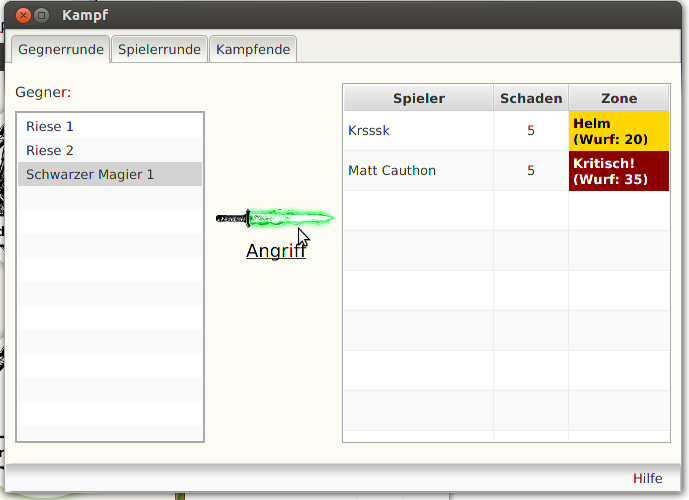
\includegraphics[width=.7\linewidth]{Bilder/Gegnerrunde.png}
\caption{Die Gegnerrunde}
\end{figure}
\subsection{Die Spielerrunde}\label{Abschnitt:Spielerrunde}
\begin{figure}
\centering
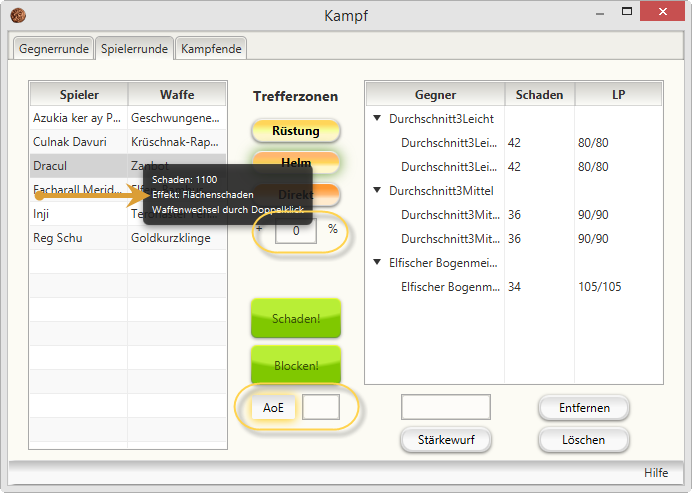
\includegraphics[width=\linewidth]{Bilder/Spielerrunde.png}
\caption{Die Spielerrunde. Markiert sind das Bonustextfeld und die zusätzlichen Elemente, die für den 'Schadet allen Gegnern'-Effekt  erscheinen.}
\label{Bild:Spielerrunde}
\end{figure}
Im Groben ist die Spielerrunde wie die Gegnerrunde aufgebaut: Links ist eine Tabelle der aktiven Kampfteilnehmer, also der Spielercharaktere. Rechts werden die Gegner angezeigt. Zusätzlich zum Schaden werden auch die aktuellen Lebenspunkte des Gegners angezeigt.

\subsubsection{Der Standardkampfablauf}\label{Abschnitt:standardkampf}
\textbf{Angriff eines Spielers.} Um anzugreifen, wird der angreifende Spielercharakter selektiert. Je nachdem, was der Spieler gewürfelt hat, kann nun einer der drei Trefferzone-Buttons geklickt werden. Besitzt der Spieler aus irgendeinem Grund einen Bonus, kann dieser vorher im Bonustextfeld spezifiziert werden, siehe Abbildung \ref{Bild:Spielerrunde}. Dann wird mithilfe der ausgewählten Waffe und der Rüstung der Gegner für jeden Gegner berechnet, wie viel Schaden dieser Angriff verursachen würde.\\

\textbf{Blocken.} Blockversuche der Gegner können mit dem großen grünen 'Blocken!'-Knopf gestartet werden. Sofort versuchen alle Gegner, zu blocken. Sind sie erfolgreich, wird 'Schaden' bei diesen Gegnern auf 0 gesetzt. Es kann mehrmals geblockt werden. Ist in der rechten Tabelle ein Spieler ausgewählt, der einen Geschickmalus hat, wird dieser beim Blocken einberechnet.\\

\textbf{Lebenspunkte reduzieren.} Durch Auswählen eines Gegners und einen Klick auf den großen grünen 'Schaden!'-Button werden die Punkte des Gegners, die in der Spalte 'Schaden' stehen, von seinen LP abgezogen. Sinken die LP auf 0, wird der Gegner direkt aus der Spieler- und Gegnerrunde entfernt. Alternativ kann die LP-Spalte durch Klicken auch direkt editiert werden.

\subsubsection{Manuelles 'Töten'}

\textbf{Um einen Gegner manuell aus dem Kampf zu entfernen,} kann man ihn auswählen und entweder auf den \textbf{Entfernen}- oder \textbf{Löschen}-Button klicken. Der 'Entfernen'-Button wirkt genauso, als hätte man die LP auf 0 gesetzt. Im Fall des 'Löschen'-Buttons wird der Gegner komplett aus dem Kampf entfernt, d.h. er zählt nicht für Erfahrungspunkte und gibt auch keine Beute.

\subsubsection{Stärkewurf}\label{Abschnitt:staerkewurf}
Unter der Gegnertabelle findet sich die Möglichkeit eines Stärkewurfs. Dazu wird der gewünscht Gegner selektiert und 'Stärkewurf' gedrückt. Das Ergebnis erscheint in dem darüber liegenden Textfeld. Ist in der linken Tabelle ein Spielercharakter selektiert, der einen Stärkemalus-Effekt hat, wird dieser mit einberechnet.

\subsubsection{Waffenwechsel}
Um die \textbf{Waffe eines Spielers zu wechseln}, reicht ein Doppelklick auf diese Waffe. Es öffnet sich ein Fenster, welches alle Waffen des Spielers sowie deren Schaden und Effekt anzeigt. Dort kann eine neue Waffe gewählt werden.

\subsubsection{Schaden auf allen Gegnern / AoE}\label{Abschnitt:aoe}
Hat eine ausgewählte Waffe den \textbf{'Schadet allen Gegnern'-Effekt}, so erscheint zusätzlich der 'AoE'-Button und ein Textfeld, siehe Abbildung \ref{Bild:Spielerrunde}. In das Textfeld kann ein Schadenswert eingetragen werden. Dann verursacht ein Klick auf 'AoE', dass jeder Gegner mit diesem Schaden angegriffen wird, bei entsprechendem Effekt auch rüstungsunabhängig. Der Schaden wird direkt von den LP subtrahiert. Gegner, deren LP auf 0 gesunken sind, werden aus der Tabelle entfernt.

\subsection{Das Kampfende}\label{Abschnitt:Kampfende}
Das Kampfende ist zuständig für \textbf{Erfahrungspunkte und Beute}.\\
Es gliedert sich in 3 Bereiche: Im linken oberen Bereich finden sich alle Gegner, die nicht in der Spielerrunde gelöscht wurden, und in der Tabelle daneben die Summe an Erfahrungspunkten, die sie bringen. Im rechten oberen Bereich wird die Beute des selektierten Gegners angezeigt, und im unteren Bereich kann diese Beute (neu) generiert werden.\\
\begin{figure}
\centering
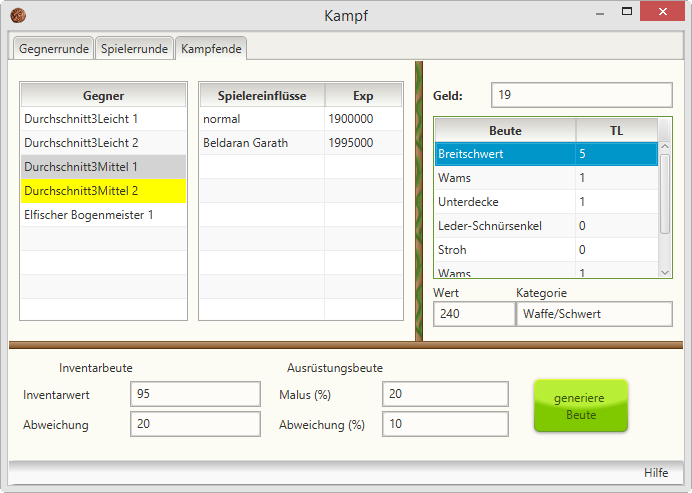
\includegraphics[width=\linewidth]{Bilder/Kampfende.png}
\caption{Das Kampfende. Man sieht einen gelb markierten Gegner.}
\label{Bild:Kampfende}
\end{figure}

Die \textbf{gelb markierten} Gegner sind die mit 0 Lebenspunkten, also jene, die nicht mehr aktiv am Kampf teilnehmen.\\

\textbf{Die Erfahrungspunkte} können durch den 'Mehr Erfahrung'-Rüstungseffekt vergrößert werden. Alle Spielercharaktere, die einen solchen Effekt besitzen, werden einzeln in der Tabelle aufgeführt, siehe Abbildung \ref{Bild:Kampfende}. Ansonsten gilt die Zahl bei 'Normal'.\\

\textbf{Die Beutetabelle} zeigt jeweils den Namen der Beute und ihre Traglast. Wird eine Beute ausgewählt, erscheinen unten zusätzlich der Wert (nur sinnvoll bei Waffen oder Rüstung) und ihre Kategorie. Zusätzlich kann auch Geld Beute sein; dieses wird überhalb der Tabelle angezeigt. Anfangs ist die Beutetabelle für jeden Gegner leer. \textbf{Damit Beute zu sehen ist}, muss sie vorher generiert werden. Selektiert man den Gegner später ein zweites Mal, sieht man immer noch dieselbe Beute.

\subsubsection{Generierung der Beute}\label{Abschnitt:Beute}
Die Beute teilt sich auf in \textbf{Inventarbeute} und \textbf{Ausrüstungsbeute}. Wie gut die Beute ist, kann durch die Textfelder im unteren Teil des Kampfende-Fensters bestimmt werden, bevor mit 'generiere Beute' Beute für den ausgewählten Gegner generiert wird.\\

Die angezeigten \textbf{Beutegegenstände kommen aus den Händler-Daten}. Möchte man also sinnvolle Beute, muss vorher der Händler aufgefüllt werden, siehe Abschnitt \ref{Abschnitt:Haendler}.\\

Für die Beute sind folgende Kategorien des Händlers wichtig: \begin{itemize}
\item Rüstung
\item Waffen
\item Handschuh bzw. Handschuhe
\item Schuh bzw. Schuhe
\item Gürtel
\item Harnisch
\item Helm
\end{itemize}
Welche Kategorie für welche Generierung wie beeinflusst, wird in den folgenden Abschnitten erläutert.\\ \\
\textbf{Generierung der Inventarbeute}\\

Inventarbeute kann aus allen Kategorien außer 'Rüstung' und 'Waffen' stammen. Das Geld zählt ebenfalls als Inventarbeute.\\

\textbf{Der Inventarwert} legt fest, wie viel die Inventarbeute wert sein soll. Dabei hat ein Geld einen Wert von 1, und ein Gegenstand den Wert, den er laut Händler kostet. Gegenstände, die 0 kosten, haben ebenfalls Wert 1.\\

\textbf{Eine Abweichung} von mehr als 0 erlaubt es, dass der Wert der Beute zwar wahrscheinlich in der Nähe des Inventarwerts liegt, aber schwankt.\footnote{Für die, die es genau wissen wollen: Es handelt sich um eine Gaußverteilung mit Erwartungswert des Inventarwerts und Varianz der Abweichung.} Dabei legt die Abweichung die ungefähre Schwankung fest.\\

Wie \textbf{groß der Anteil des Geldes an der Inventarbeute} ist, wird zufällig bestimmt.\\
\clearpage
\textbf{Generierung der Ausrüstungsbeute}\\

Ausrüstungsbeute stammt nur aus den Kategorien 'Rüstung' und 'Waffen'. 
Die Parameter für die Generierung der Ausrüstungsbeute sind ähnlich zu denen des Inventars:\\

\textbf{Der Malus} legt fest, wie gut die Ausrüstung ist. Dabei sagt er prozentual, wie viel schlechter sie sein soll als die tatsächliche Ausrüstung des Gegners. Dabei wird bei der Rüstung davon ausgegangen, dass der Harnisch 50\% von DefR ausmacht und Schuh, Gürtel und Handschuhe zu gleichen Teilen den Rest.\\

\textbf{Die Streuung} funktioniert ebenso für den Malus wie die Abweichung für den Inventarwert.\\

Der Gegner lässt mit unterschiedlichen Wahrscheinlichkeiten die verschiedenen Teile seiner Ausrüstung fallen:\\
\begin{center}
\begin{tabular}{c|c}
Kategorie & Wahrscheinlichkeit\\
\hline
Waffe & 40\% \\
Helm & 12\% \\
Harnisch & 12\% \\
Schuhe & 12\% \\
Handschuhe & 12\% \\
Gürtel & 12\% \\
\end{tabular}
\end{center}
Gibt es die entsprechende Kategorie nicht im Händler, kann es sein, dass kein Ausrüstungsteil in der Beute vorkommt.

\clearpage
\section{Händler (Giakiri, der Händler)}\label{Abschnitt:Haendler}
Im Händler können Gegenstände kategorisiert und gesucht werden. Auch für eine sinnvolle Beutegenerierung ist der Händler unerlässlich, siehe Abschnitt \ref{Abschnitt:Beute}.\\
Grob teilt sich der Händler in die beiden Tabs \textbf{Einfache Gegenstände} und \textbf{Rüstung/Waffen}.
Diese Aufteilung ergibt sich daraus, dass Rüstung und Waffen zusätzlich noch einen Wert und eine benötigte Stärke brauchen.
\begin{figure}
\centering
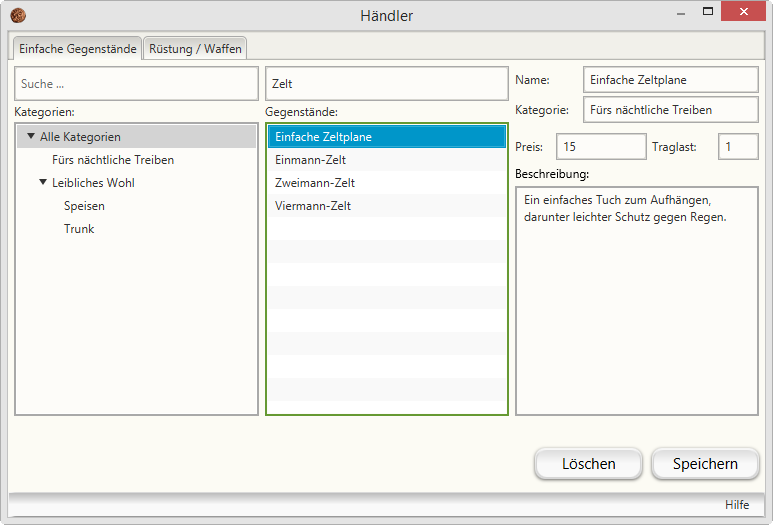
\includegraphics[width=1\linewidth]{Bilder/InventarHaendler.png}
\caption{Der Inventar-Händler}
\label{fig:Inventarhaendler}
\end{figure}
\subsection{Allgemein}
Die beiden Tabs sind von Aussehen und Bedienung annähernd gleich.\\

\textbf{Ein Gegenstand kann hinzufügt werden}, indem wie üblich auf 'Neuer Gegenstand' geklickt wird, dessen Werte editiert werden und dann entweder 'Enter' gedrückt wird oder auf 'Speichern' geklickt wird. \\
Für das erstellen in einer neue (Sub-)Kategorie siehe weiter unten 'Neue Kategorien'. Um den Gegenstand einer vorhandenen Kategorie hinzuzufügen kann entweder einfach der komplette Name (mit Oberkategorien) der \\(Sub-)Kategorie hineingeschrieben werden oder die gewünschte Kategorie in der Kategorieliste ausgewählt werden (und dann erneut neuer Gegenstand).\\

\textbf{Gegenstände editieren} funktioniert genauso wie Gegenstände hinzufügen, nur, dass der zu editierende Gegenstand auszuwählen ist.\\

Es gibt zwei Möglichkeiten, \textbf{Gegenstände zu suchen}. Entweder, man nutzt das Suchfeld über der Gegenstandsliste. In diesem Fall werden die Gegenstände aller Kategorien durchsucht. Oder man weiß bereits, in welcher Kategorie sich ein Gegenstand befindet. Dann kann man nach der entsprechenden Kategorie über der Kategorieliste suchen und sie dann auswählen, um alle Gegenstände dieser Kategorie zu sehen. \\

\textbf{Gegenstände} können \textbf{gelöscht} werden, indem sie ausgewählt und mit dem 'Löschen'-Button entfernt werden.\\

\textbf{Neue Kategorien} werden automatisch angelegt, wenn man sie für einen Gegenstand festlegt. Dabei bedeutet z.B. 'Rüstung/Handschuh/Eiserner Handschuh', dass das Objekt in der Kategorie 'Eiserner Handschuh' ist, die wiederum eine Unterkategorie von 'Handschuh' ist, was wiederum eine Unterkategorie von 'Rüstung' ist.\\

\textbf{Kategorien löschen}. Kategorien werden automatisch entfernt, wenn es keine Gegenstände dieser Kategorie mehr gibt. Dies ist allerdings erst bei Neustart des Händlers ersichtlich.

\subsection{Rüstung und Waffen}
\begin{figure}
\centering
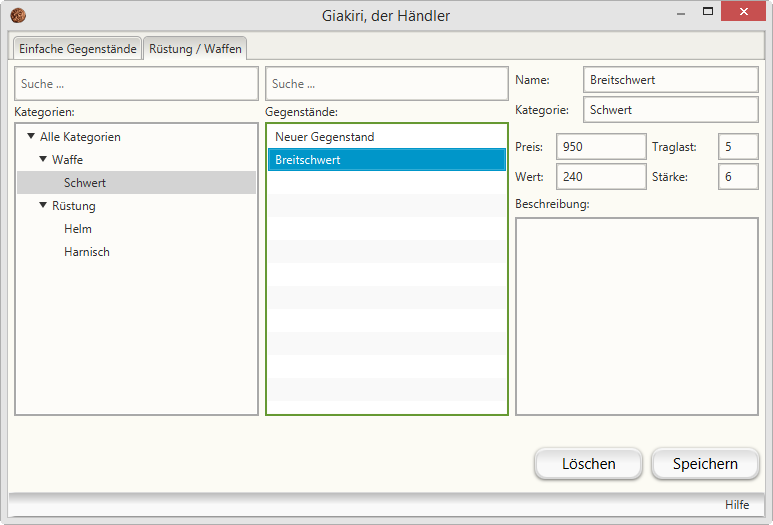
\includegraphics[width=.8\linewidth]{Bilder/AusruestungsHaendler.png}
\caption{Der Ausrüstungs-Händler}
\label{fig:Ausruestungshaendler}
\end{figure}

Rüstung und Waffen besitzen im Gegensatz zu anderen Gegenständen die Eigenschaften der benötigten Stärke und des Wertes, siehe Abbildung \ref{fig:Ausruestungshaendler}.

\clearpage
\section{Würfeln (Ceto, der Würfelspieler)}
Sehr einfache Funktionalität, die es erlaubt, \textbf{beliebige Würfelwürfe} zu simulieren.
\begin{figure}
\centering
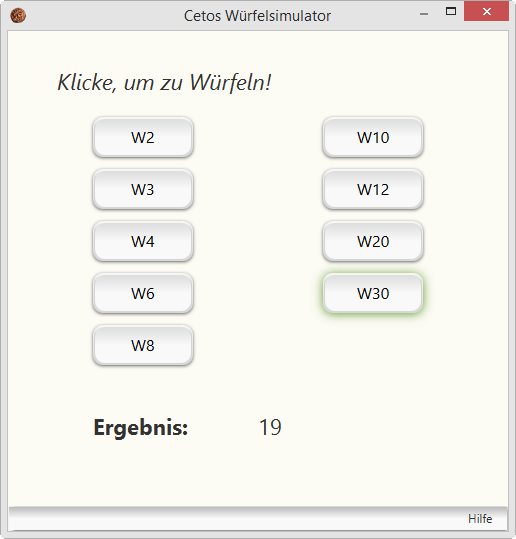
\includegraphics[width=.8\linewidth]{Bilder/wuerfeln.png}
\caption{9 verschiedene Würfel im Würfelspieler}
\end{figure}
\end{document}